\chapter{引言}
\label{cha:intro}

\section{研究背景}
\label{sec:background}
互联网的出现使人与人之间的交流变得简单轻松,信息交流更加便捷,各种各样的网络服务层出不穷,共享单车、网约车和在线教育就在很短的时间内让人们的生活发生了很大的改变。人们都频繁在网上获取信息,并寻找更加优质的服务。因此,它很大程度上改变了人们的生活方式,让人们的生活变得丰富多彩。第41次《中国互联网络发展状况统计报告》\cite{networkreport}指出,截至 2018年6月,我国网民规模已达到了8.02亿,半年之内我国新增2968万网民,每天平均几乎有16万新网民加入互联网,我国的互联网已经成为很多人必不可少的一部分。不仅仅是人们生活实用互联网频率不断增加,很多企业也使用互联网管理设备和存储用户信息。

在这种情况下,网络安全问题就会对我们的社会造成极大的损失。有很多网络非法行为给人们造成了很多损失。2018年8月3日,台积电(TSMC)被病毒Wannacry病毒入侵,它的基地生产线摆停。虽然最后病毒被成功清理,但是台积电也因此预计造成约17.6亿元人民币损失。同年8月28日,华住酒店信息泄露,其中涉及姓名、身份证号、邮箱、家庭住址、开房记录等敏感信息约5亿条被出售。

网络安全问题需要被重视,因为网络安全问题很可能会造成不必要的损失。在众多网络安全攻击中,拒绝服务攻击(Denial of Service, DoS)攻击作为一种普遍而又威力强大的攻击,被黑客广泛的使用,对互联网的系统造成了极大的危害。而分布式拒绝服务攻击(Distributed Denail of Service, DDoS)作为DoS攻击的新模式,它拥有更加强大的攻击威力和更好的隐蔽性,使无数的企业都为该类攻击所困扰。


2018年1月29日, DDoS攻击迫使荷兰三大银行(荷兰银行、荷兰合作银行和ING银行)的服务器超载。因此,它们网站和互联网银行服务瘫痪,荷兰税务局也遭受到类似的处境。
% http://www.sohu.com/a/272186665_100238920

2018年2月28日,世界上最顶尖的代码托管网站Github遭受了DDoS攻击并因此在几分钟内无法提供正常的服务,使很多公司都收到了影响。该攻击的峰值速率高达1.35Tb/s,超过了以往的所有DDoS峰值速率记录记录。
% http://www.sohu.com/a/272186665_100238920

2018年4月17日,美国的网络安全服务运营商Sucuri也遭受了大规模的DDoS攻击,导致一些端口的吞吐量达到容量上限,因此有非常高的延迟甚至还出现了数据包的丢失。因此,在西欧、南美和美国东部部分地区的服务被迫中断。
% http://www.cert.org.cn/publish/main/98/2018/20180426085352471430574/20180426085352471430574_.html

2018年5月13日,丹麦的铁路运营商(DSB)的系统受到了DDoS攻击,该公司的售票机、商店还有旅客的手机客户端都无法完成购票流程。因此,该公司不得不采用人工售票的方式暂时缓解压力,直到5月14日上午才能得到解决。这次事件让1.5万旅客受到了影响。
%http://www.cert.org.cn/publish/main/98/2018/20180518143816118933026/20180518143816118933026_.html

在卡巴斯基实验室2018年第四季度的调查中,我国的网络安全形势依然不容更乐观,中国依然是全世界范围内受DDoS攻击最严重的国家,所以,我们需要重视DDoS的防御问题。
% https://securelist.com/ddos-attacks-in-q4-2018/89565/

\begin{figure}
    \centering
    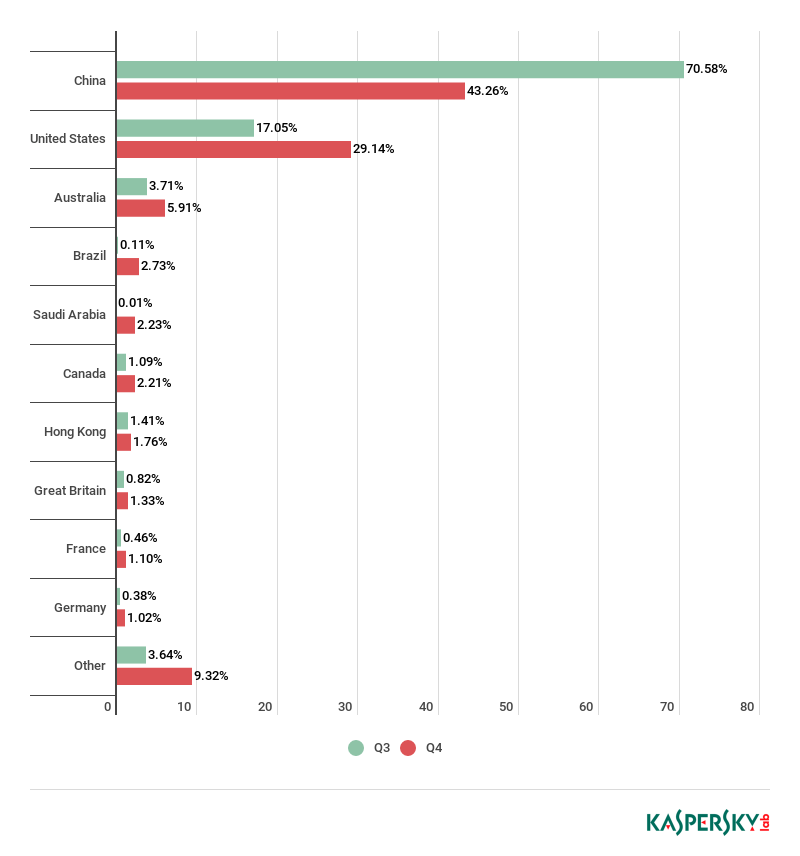
\includegraphics[scale=0.5]{figures/en-ddos-by-countries.png}
    \caption{在2018年Q3和Q4中,世界各国受DDoS攻击分布}
    \label{fig:ddos_countries}
\end{figure}

DoS攻击的危害是很大的,而且它的实现形式也是各不相同。在所有的DoS攻击种类中,低速率服务拒绝(Low-rate Denial of Service, LDoS)攻击\cite{LDoS}是一种针对良性TCP流最有效的一种攻击。和直接发送大量流量的洪泛方式不同,它通过发送周期性的脉冲低速流就可以持续迫使TCP流进入超时重传的等待阶段,造成TCP流吞吐量显著下降的可怕后果。而且由于LDoS攻击的并非洪泛的方式,平均速率很低。相对于洪泛方式的DoS攻击,LDoS攻击更加难以被检测,而且,LDoS攻击以分布式方式实现的时候,LDoS攻击的隐蔽性更加强。
% Among all kinds of DoS attacks, the low-rate TCP attack~\cite{b20} is essentially the most efficient in terms of causing damage to benign TCP flows. Instead of directly sending a huge amount of traffic, it generates periodically pulsing low-rate flows to cause continuous retransmission of benign TCP flows, which results in significant throughput degradation. Due to the low rate, such attack is more difficult to be detected compared to flooding-based attacks. Moreover, the attack can be launched in a distributed mode, which further increases its stealthiness.

目前,为了有效的防御LDoS攻击,很多相应的对抗方案已经被提出来。大部分的解决方案\cite{b1,b4, b6, b7, b22}通过使用数字信号处理(Digital Signal Processing, DSP)技术来提取频域特征。只有采集数据流的周期合适的情况下,这样的特征才能够很好的提取特征。然而,现行的方案都是采用一个固定的采样周期,来检测攻击流,这样会导致一些具有短周期的LDoS攻击流无法被检测出来。除此之外,这些方案都没有考虑如何限制被识别的攻击流。有一些方案采用被动的防御方案来缓解LDoS攻击,不过,这些方案都没有识别攻击流,这些方案包括在主机上对TCP协议栈的RTO进行随机化\cite{b17}和修改交换机上丢包机制的公平性规则\cite{b8}。因为这样的修改涉及到用户的网络协议栈或者交换机上面的硬件,所以这样的被动防御方案很难部署在大量的交换机上面。
%To effectively defend against the attack, several countermeasures have been proposed. Most defense solutions~\cite{b1,b4, b6, b7, b22} identify the attack flows by applying digital signal processing (DSP) techniques to extract frequency-domain characteristics. Such characteristics can only be well depicted when a proper sampling period of collecting flow statistics is set. However, existing methods apply a fixed sampling period, which may fail to detect attack flows with short periods. Besides, they do not consider how to throttle the identified flows. A few countermeasures adapt passive methods to mitigate the low-rate TCP attack without identifying attack flows, such as randomizing RTO of the TCP protocol stack in hosts\cite{b17} and modifying the fairness mechanism of dropping packets in the switches \cite{b8}. The passive defense solutions are not easy to be deployed in practice due to the modification of the network protocol stack in hosts or hardware in switches.

进来,软件定义网络(Software-Defined Networking, SDN)作为一个很有潜力的新型网络出现,改变了现行的网络架构的限制。首先,SDN网络将网络的控制平面从下层的路由器和交换机中分离出来,这样下层的交换机只需要负责数据平面,即转发数据流。其次,通过将数据平面和控制平面分离,SDN将控制逻辑放在中心控制器上,而交换机则负责数据的转发,这能够较为简单的配置网络和执行新的网络策略。而且,由于交换机只要与控制器完成连接,就可以接入已有网络并且不需要重复配置就能够执行统一的策略。



\begin{figure}
    \centering
    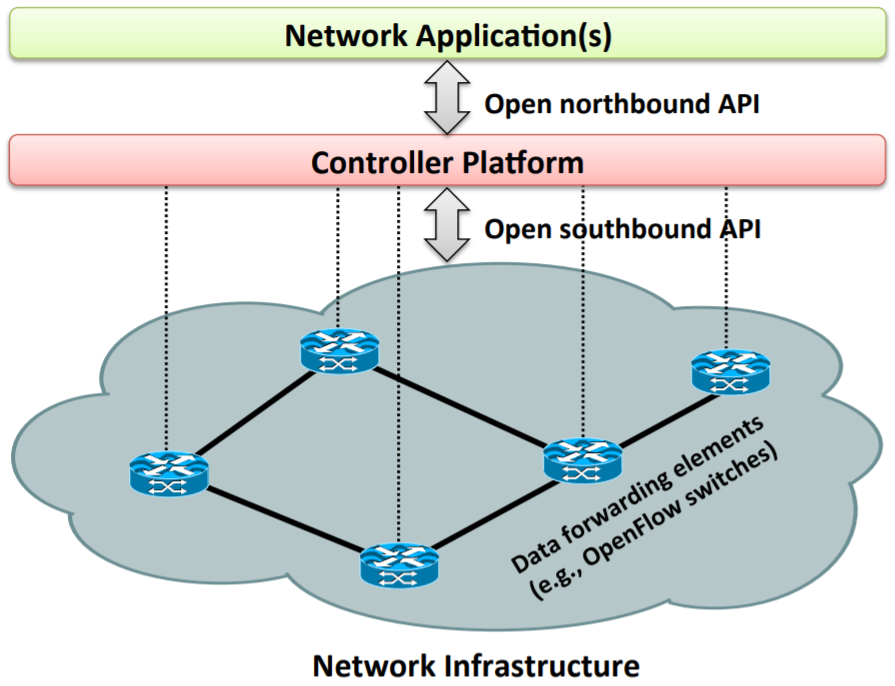
\includegraphics[scale=0.5]{figures/SDNnetwork.png}
    \caption{SDN网络架构}
    \label{fig:sdnfig}
\end{figure}

由于SDN是中心控制网络,控制平面和转发平面分离,所以通过编程灵活地制定网络安全策略能够达到比传统网络更加好的效果。,所以,它在对抗DoS攻击上面有很多的优势。很多基于SDN实现的方案~\cite{b9, b16, b11, b23, b24}被踢出来防御各种各样的DoS攻击。但是,已有的方案都将注意力集中在防御洪泛式的DoS攻击。他们都没有考虑到如何检测和缓解LDoS攻击。值得注意的是,LDoS攻击的攻击流特点与洪泛式攻击的特点是有很大差别的。
%Recently, Software-Defined Networking (SDN) has emerged as a promising network paradigm. Due to the centralized control and flexible programmability, it shows great benefits on defeating DoS attacks. Several SDN-based approaches~\cite{b9, b16, b11, b23, b24} have been proposed to defend against various DoS attacks. However, existing defenses focus on defeating flooding-based DoS attacks. They fail to consider how to detect and mitigate the low-rate TCP attack. Now that the attack has great differences on the characteristics of the attack flows compared to the flooding attacks.

综上所述,LDoS攻击防御的问题还是需要去研究的。因为,在之前的工作中,传统网络的LDoS攻击的防御方案都有着其固有的缺陷,有的方案定位并且限制LDoS攻击源。有的方案需要对交换机或者主机进行比较大的修改。而且当新的设备接入网络的时候需要重新配置,相对比较复杂。而已有的SDN的DoS防御方案没有针对于LDoS攻击的相关研究。相较于之前的LDoS防御方案,基于SDN的LDoS防御方案能够拥有更好的效果。

\section{主要研究内容}
\label{sec:work}
本文中的研究的主要内容是SDN网络的安全问题,针对DoS攻击的特殊攻击方式LDoS攻击的防御机制进行研究。在SDN网络环境下,完成了一种基于周期性的LDoS攻击防御系统。该系统在针对LDoS攻击有不错的表现,无论是准确率还是误判率都达到很好的效果,同时,引入该系统的开销也很低。本文在真实的SDN网络交换机上完成实验,并且对系统进行了评估。

本文首先介绍LDoS攻击防御的研究现状,然后对现行的SDN中的DoS攻击防御的研究进展进行讨论。通过分析LDoS攻击的特点,平均速率很低、瞬时速率很高、具有周期性的特点设计相应的防御方案,提出了两个方案来抵御LDoS攻击。第一种策略是使用带宽保障策略来保证TCP传输的所需要的最低带宽保障;第二种策略是限制攻击源的方式,提出了基于周期性检测的LDoS攻击检测算法和基于平均欧式距离(Mean Euclidean Distance, MED)的恶意流判定算法,再利用SDN的全局视野,可以很快的找到攻击源,并对攻击源进行限制。


\section{主要贡献}
\label{sec:contribution}
总结一下,本文的四个主要贡献点:

\begin{itemize}
    \item 本文提出了一个防御系统,它能够有效地防御LDoS攻击而且不需要对交换机或者协议做任何修改
    \item 本文提出了一种策略能够保证良性TCP流的传输,能够保证TCP流传输的最低保障
    \item 本文提出了精准识别LDoS恶意攻击流的算法,能够准确地识别攻击源
    \item 本文在Floodlight控制器上实现了真实的SDN网络实验并做实验验证了本文防御系统的有效性
\end{itemize}

\section{文章内容安排}
\label{sec:arrange}

